% --------------------------------------------------------------
% This is all preamble stuff that you don't have to worry about.
% Head down to where it says "Start here"
% --------------------------------------------------------------
 
\documentclass[12pt]{article}
 
\usepackage[margin=1in]{geometry} 
\usepackage{graphicx}
\usepackage{amsmath,amsthm,amssymb}
\usepackage{xcolor}
\usepackage{url}
\usepackage{hyperref}
\newcommand{\N}{\mathbb{N}}
\newcommand{\Z}{\mathbb{Z}}
\newcommand{\comment}[1]{}
\usepackage{float}
\usepackage[export]{adjustbox}
\usepackage{listings}

\newenvironment{theorem}[2][Theorem]{\begin{trivlist}
\item[\hskip \labelsep {\bfseries #1}\hskip \labelsep {\bfseries #2.}]}{\end{trivlist}}
\newenvironment{lemma}[2][Lemma]{\begin{trivlist}
\item[\hskip \labelsep {\bfseries #1}\hskip \labelsep {\bfseries #2.}]}{\end{trivlist}}
\newenvironment{exercise}[2][Exercise]{\begin{trivlist}
\item[\hskip \labelsep {\bfseries #1}\hskip \labelsep {\bfseries #2.}]}{\end{trivlist}}
\newenvironment{problem}[2][Problem]{\begin{trivlist}
\item[\hskip \labelsep {\bfseries #1}\hskip \labelsep {\bfseries #2.}]}{\end{trivlist}}
\newenvironment{question}[2][Question]{\begin{trivlist}
\item[\hskip \labelsep {\bfseries #1}\hskip \labelsep {\bfseries #2.}]}{\end{trivlist}}
\newenvironment{corollary}[2][Corollary]{\begin{trivlist}
\item[\hskip \labelsep {\bfseries #1}\hskip \labelsep {\bfseries #2.}]}{\end{trivlist}}

\newenvironment{solution}{\begin{proof}[Solution]}{\end{proof}}
 
\begin{document}

 
% --------------------------------------------------------------
%                         Start here
% --------------------------------------------------------------
 
\title{Assignment 3}
\author{CS330: Operating Systems}
\date{}

\maketitle

\section{Introduction}

As part of this assignment,
you will be implementing system calls in a teaching OS (gemOS), same as in Assignment-2. 
%
We will be using a minimal OS called gemOS to implement these system calls and provide system call APIs to the user space. 
%
The gemOS source can be found in the {\tt src} directory. This source provides the OS source code and the user space 
process (i.e., {\tt init} process) code (in {\tt src/user} directory).

gemOS is a teaching operating system. Typically OS boots on a hardware. To set up the gemOS, you can refer to the document ({\tt Documentation/gemOS\_Setup.pdf})
\comment{
 An architectural simulator simulates the hardware in software. 
%
In other words, all the hardware functionalities are implemented in software using some programming language. 
%
For example, Gem5 simulator implements architectural elements for different architectures like
ARM, X86, MIPS etc.
%
Advantages of using software simulators for OS development are,
\begin{itemize}
\item Internal hardware state and operations at different components (e.g., decoder, cache etc.) can be
profiled to better understand the hardware-software interfacing.
\item Hardware can be modified for several purposes---make it simpler, understand implications of 
hardware changes on software design etc.
\item Bugs during OS development can be better understood by debugging both hardware code and the OS code.     
\end{itemize} 
%
The getting started guide helps you to setup Gem5 and execute \texttt{gemOS} on it. 
You can refer to \href{http://learning.gem5.org/book/index.html}{this} online tutorial to know more about gem5.\\


You need to setup gem5 by following the instructions (Step-0) mentioned in Section~\ref{sec:s0}. 
We suggest to complete \textbf{Step-0} immediately to have a working gem5 simulator to start with 
the assignment. \textbf{Step-0} also helps you to understand how to boot \textbf{gemOS} binary in gem5. 
You can build the gemOS source provided in the {\tt src} directory to test the working. 

The assignment is divided into five tasks. The implementation of system calls for each task should be POSIX compliant. 
Which means, you need to read the man pages of each of corresponding system calls to know about their exact behavior. 
Testing procedure and submission guidelines are mentioned at the end of the document. 

\section{Step-0: Getting Ready}
\label{sec:s0}

This section explains the setup procedure of gem5. Further, it explains the process to build and execute gemOS 
on gem5 platform and access the terminal to see the messages printed by the gemOS.

\subsection{Preparing Gem5 simulator}
\subsubsection*{System pre-requisites}
\begin{itemize}
    \item Git
    \item gcc 4.8+
    \item python 2.7+
    \item SCons
    \item protobuf 2.1+
\end{itemize}
\begin{flushleft}
On Ubuntu install the packages by executing the following command. 

\vspace{0.25cm}
\noindent
\texttt{\$ sudo apt-get install build-essential git m4 scons zlib1g zlib1g-dev libprotobuf-dev protobuf-compiler libprotoc-dev  libgoogle-perftools-dev python-dev python automake}
\end{flushleft} 
\vspace{5mm}
\subsubsection*{Gem5 installation} 
Clone the gem5 repository from \url{https://gem5.googlesource.com/public/gem5}.

\vspace{0.25cm}
\noindent
\texttt{\$ git clone https://gem5.googlesource.com/public/gem5}

\vspace{0.25cm}
\noindent
Change the current directory to \texttt{gem5} and build it with scons:

\vspace{0.25cm}
\noindent
\texttt{\$ cd gem5 \\
 \$ scons build/X86/gem5.opt -j9}

\vspace{0.25cm}
\noindent
In place of 9 in [-j9], you can use a number equal to available cores in your system plus one. 
For example, if your system have 4 cores, then substitute -j9 with -j5. 
For first time it will take around 10 to 30 minutes depending on your system configuration. 
After a successful Gem5 build, test it using the following command,


\vspace{0.25cm}
\noindent
\texttt{\$ \small{build/X86/gem5.opt configs/example/se.py --cmd=tests/test-progs/hello/bin/x86/linux/hello}}

\vspace{0.25cm}
\noindent
The output should be as follows,
\begin{footnotesize}
\begin{verbatim}
 gem5 Simulator System.  http://gem5.org
 gem5 is copyrighted software; use the --copyright option for details.
 gem5 compiled Aug  4 2018 11:00:44
 gem5 started Aug  4 2018 17:15:06
 gem5 executing on BM1AF-BP1AF-BM6AF, pid 8965
 command line: build/X86/gem5.opt configs/example/se.py \
               --cmd=tests/test-progs/hello/bin/x86/linux/hello
 /home/user/workspace/gem5/configs/common/CacheConfig.py:50: SyntaxWarning: import * only \ 
               allowed at module level def config_cache(options, system):
 Global frequency set at 1000000000000 ticks per second
 warn: DRAM device capacity (8192 Mbytes) does not match the address range assigned (512 Mbytes)
 0: system.remote_gdb: listening for remote gdb on port 7000
 **** REAL SIMULATION ****
 info: Entering event queue @ 0. Starting simulation.....
 Hello world!
 Exiting @ tick 5941500 because exiting with last active thread context 
\end{verbatim}
\end{footnotesize}

\subsection{Booting gemOS using Gem5} 
Gem5 execute in two modes---system call emulation (SE) mode and full system (FS) simulation mode.
%
The example shown in the previous section, was a SE mode simulation of Gem5 to execute an application.
%
As we want to execute an OS, Gem5 should be executed in FS mode. 
%
There are some initial setup to do before we can execute \texttt{gemOS} using Gem5 FS mode.
%
To run OS in full-system mode, where we are required to simulate the hardware in detail, 
we need to provide the following files,
\begin{itemize}
    \item \texttt{gemOS.kernel}: OS binary built from the \texttt{gemOS} source. 
    \item \texttt{gemOS.img}: root disk image
    \item \texttt{swap.img}: swap disk image
\end{itemize}

Gem5 is required to be properly configured to execute the \texttt{gemOS} kernel. 
The configuration requires changing
some existing configuration files (in gem5 directory) as follows,
\begin{itemize}
   \item Edit the \texttt{configs/common/FSConfig.py} file to modify the \texttt{makeX86System} function
         where the value of \texttt{disk2.childImage} is modified to \texttt{(disk('swap.img'))}.
   \item Edit the \texttt{configs/common/Benchmarks.py} file to update it as follows, 
         \begin{verbatim}
             elif buildEnv['TARGET_ISA'] == 'x86':
                   return env.get('LINUX_IMAGE', disk('gemOS.img'))
         \end{verbatim}
\end{itemize}
\noindent
Create a directory named \texttt{gemos} in \texttt{gem5} directory and populate it as follows,

\vspace{0.25cm}
\noindent
\texttt{/home/user/gem5\$ mkdir gemos} \\
\texttt{/home/user/gem5\$ cd gemos} \\
\texttt{/home/user/gem5/gemos\$ mkdir disks; mkdir binaries} \\
\texttt{/home/user/gem5/gemos\$ dd if=/dev/zero of=disks/gemOS.img bs=1M count=128} \\
\texttt{/home/user/gem5/gemos\$ dd if=/dev/zero of=disks/swap.img bs=1M count=32} \\



%
For the time being, you can use \texttt{gemOS.kernel} provided with the assignment (can be found in {\tt src} directory). 
Copy the \texttt{gemOS.kernel} to {\tt gemos/binaries} directory.\\
%
We need to set the \texttt{M5\_PATH} environment variable to the \texttt{gemos} directory path as follows,


\vspace{0.25cm}
\noindent
\texttt{/home/user/gem5\$ export M5\_PATH=/home/user/gem5/gemos}
 
\vspace{0.25cm}
\noindent
Now, we are ready to boot GemOS.

\vspace{0.25cm}
\noindent
\texttt{gem5\$ build/X86/gem5.opt configs/example/fs.py} \\ {\tt --kernel=/home/user/gem5/gemos/binaries/gemOS.kernel --mem-size=2048MB}

\vspace{0.25cm}
\noindent
gem5 output will look as follows,
\begin{scriptsize}
\begin{verbatim}
gem5 Simulator System.  http://gem5.org
gem5 is copyrighted software; use the --copyright option for details.

gem5 compiled Aug 21 2019 23:45:13
gem5 started Aug 22 2019 10:45:01
gem5 executing on kparun-BM1AF-BP1AF-BM6AF, pid 28942
command line: build/X86/gem5.opt configs/example/fs.py --kernel=/home/kparun/gem5/gemos/binaries/gemOS.kernel --mem-size=2048MB

Global frequency set at 1000000000000 ticks per second
warn: DRAM device capacity (8192 Mbytes) does not match the address range assigned (512 Mbytes)
info: kernel located at: /home/kparun/gem5/gemos/binaries/gemOS.kernel
system.pc.com_1.device: Listening for connections on port 3456
      0: rtc: Real-time clock set to Sun Jan  1 00:00:00 2012
0: system.remote_gdb: listening for remote gdb on port 7000
warn: Reading current count from inactive timer.
**** REAL SIMULATION ****
info: Entering event queue @ 0.  Starting simulation...
warn: Don't know what interrupt to clear for console.
\end{verbatim} 
\end{scriptsize}
\noindent
Execute the following command in another terminal window to access the \texttt{gemOS} console 

\vspace{0.25cm}
\noindent
\texttt{/home/user\$ telnet localhost 3456}


\vspace{0.25cm}
\noindent
At this point, you should be able to see the \texttt{gemOS} shell. 

\subsection{How to build gemOS}

To build \textbf{gemOS.kernel}, you need to run \textbf{make} inside \textbf{src} folder. 
After that you need to copy \textbf{gemOS.kernel} binary to \texttt{gemos/binaries} directory. 
This step is necessary every time you build the gemOS and want to test it.
After copying \texttt{gemOS.kernel}, run\\ \newline

\vspace{0.25cm}
\noindent
\texttt{gem5\$ build/X86/gem5.opt configs/example/fs.py} \\ {\tt --kernel=/home/user/gem5/gemos/binaries/gemOS.kernel --mem-size=2048MB}
\vspace{0.25cm}

\noindent
Open a terminal window as before and access the console using the following command, \\

\noindent
\texttt{/home/user\$ telnet localhost 3456}.

\subsection{How to test your Implementation}

In the \textbf{GemOS\#} terminal (accessed using the {\tt telnet} command as shown above),
you can type \textbf{init} to execute the user space process i.e, {\tt init}. 
The user space code is available in {\tt src/user/init.c}. Three user space files are used to implement the
user space logic. They are
\begin{itemize}
    \item[{\tt init.c}:] Implements the first user space process which can invoke {\tt fork()} to create more processes. Note that, there
    is no {\tt exec} system call yet in the version provided to you. For changing the user space logic, you are required to modify {\em only} 
    {\tt init.c}.
\item[{\tt lib.c}:] Implements system call wrappers and provide different user space libraries (e.g., {\tt printf}). 
    Note that you {\em do not} modify this file.
\item[{\tt lib.c}:] Provides declarations of macros and functions.
    Note that you {\em do not} modify this file.
\end{itemize}

You need to write your test cases in \textbf{init.c} to validate your implementation. The sample test-cases (in {\tt src/user/test\_cases/testcase*.c})
can be copied into {\tt init.c} to make use of them. If your implementation is correct, the output of executing test cases should match the 
expected output provided in {\tt src/user/test\_cases/testcase*.output}. 
The user and kernel code are compiled into a single binary file, i.e., \textbf{gemOS.kernel} when built using {\tt make} from 
the {\tt src} directory.
}
\section*{The Syscalls Specifications}

% The process control block (PCB) is implemented using a structure named exec\_context defined in src/include/context.h.
% As part of this assignment you will be learning how to map and unmap a virtual memory range to a process's context by implementing mmap() and munmap(). The process exec\_context contains a pointer to a linked list of struct vm\_areas. 

% You will also get acquainted with how to create a new process by forking the current process.

% The files which yo

The specifications of the systems calls that you need to implement are explained below. 

\begin{itemize}
    \item {\tt void *mmap(void *addr, size\_t length, int prot, int flags)}
    \item {\tt int munmap(void *addr, size\_t length)}
    \item {\tt int mprotect(void *addr, size\_t length, int prot)}
    \item {\tt int cfork(void)}
    \item {\tt int vfork(void)}
\end{itemize}



\newpage
\subsection *{\tt mmap(void *addr, size\_t length, int prot, int flags)}

 Creates a new mapping in the virtual address space of the calling process.  The starting address for the new mapping is specified in {\tt addr} which is page aligned. The {\tt length} argument specifies the length of the mapping (which must be greater than 0 and may not be in the multiple of page size).

	If {\tt addr} is NULL, then you have to choose a address which is page aligned in the virtual address space to create the mapping.  If {\tt addr} is not NULL, then it should be considered as a hint about where to place the mapping. If requested mappings are free, then you can either create a new mapping or merge with the existing mapping based on the scenarios explained below.
	
	\subsubsection *{\tt{Without hint address}}
	
	\begin{itemize}
	    \item Always create new mapping ({\tt vm\_area}) starting from MMAP\_AREA\_START (start) to MMAP\_AREA\_END (end). You shouldn't create new mapping in intermediate addresses unless hint address is specified. 
	    
	    \begin{figure}[H]
	    \centering
	    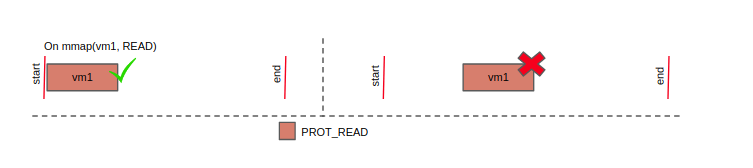
\includegraphics[scale=0.6]{mmfig1.png}
	    \label{fig:my_label}
	    \end{figure}
	    
	    \item  The subsequent mapping (new mapping) should be created in next contiguous free address in the virtual address space.
	    
	    \begin{figure}[H]
	    \centering
	    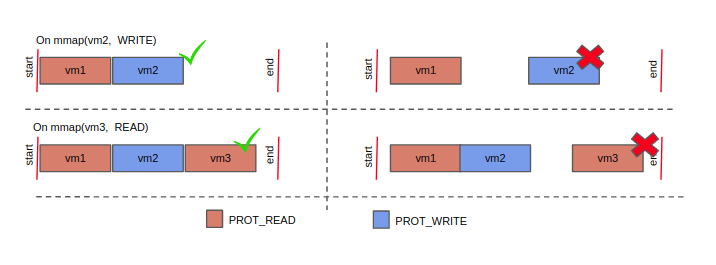
\includegraphics[scale=0.6]{mmfig2.png}
	    \label{fig:my_label}
	    \end{figure}
	    \newpage
	    \item  While merging, always choose the first immediate available free space in the virtual address space
	    
	    \begin{figure}[H]
	    \centering
	    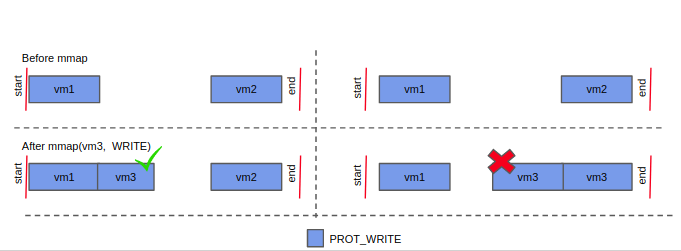
\includegraphics[scale=0.6]{mmfig3.png}
	    \label{fig:my_label}
	    \end{figure}
	\end{itemize}
	
	
	\subsubsection *{\tt{With hint address}}
	
		\begin{itemize}
	    \item When the new mapping follows the end of an existing mapping and has same protection flags as the the existing one, new mapping should be merged with the existing mapping. 
	    (Refer to case 1  in the following diagram)
	    \item  When the new mapping's end is followed by the start of an existing mapping and has same protection flags as the existing one, new mapping should be merged with the existing mapping. 
	    (Refer to the case 2 in the following diagram)
	    \item  When the new mapping cannot be merged with any of the existing mappings, a new mapping should be created (Refer to the case 3 in the following diagram)
	     \begin{figure}[H]
	    \centering
	    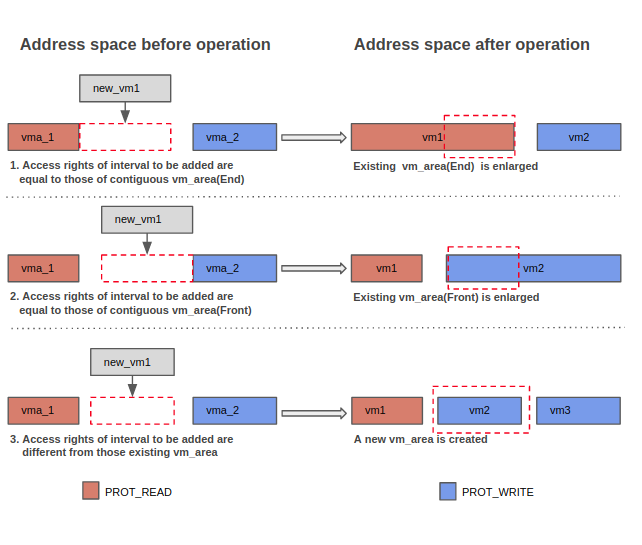
\includegraphics[scale=0.6]{mm4.png}
	    \label{fig:my_label}
	    \caption{{\tt mmap} with hint addres}
	    \end{figure}
	\end{itemize}
	
	If another mapping already exists for the provided hint address, pick a new address that may or may not depend on the hint address. You might have to create a new mappings or merge with existing mapping as mentioned in the above figure. The new address which was picked is returned as the result of the {\tt mmap} call.

	
	The {\tt prot} argument describes the desired memory protection of the mapping.  It can be bitwise OR of one or more of the following flags:
	
	\begin{itemize}
        \item {{\tt PROT\_READ}  -  The protection of the mapping ({\tt vm\_area}) is set to {\tt READ\_ONLY}. The physical pages which map to this {\tt vm\_area} are also set to {\tt READ\_ONLY}. If any process tries to write on this physical page it will result in {\tt SIGSEGV}}
        
        \item { {\tt PROT\_WRITE} - The protection of the mapping ({\tt vm\_area}) is set to {\tt WRITE\_ONLY}. When it comes to physical pages, {\tt PROT\_WRITE} implicitly provides read access to them. Hence the physical pages which map to this {\tt vm\_area} will have {\tt READ\_WRITE} access.}
        
    \end{itemize}
    The usage of {\tt flags} argument is explained below.
    
    \begin{itemize}
        \item {{\tt MAP\_FIXED} - Don't interpret addr as a hint: place the mapping at exactly that address which is passed as an argument to the mmap function.  {\tt addr} must be page-aligned and should be in the multiple of page size. If the
			specified address is already mapped with some {\tt vm\_area}. Then it cannot be used, {\tt mmap()} will fail in that case.}
         \item {{\tt MAP\_POPULATE} - Map the physical pages to the mappings({\tt vm\_area}) at the time of creation. If a mapping ({\tt vm\_area}) is created without using {\tt MAP\_POPULATE} flag. Then created mapping will not have any physical pages mapped with it. The physical pages are mapped on demand (Lazy allocation) whenever they are accessed. The access will in turn result in a page fault and then physical pages are mapped (huge overhead). }
    \end{itemize}
\subsection*{\tt RETURN VALUE}
On success, {\tt mmap()} returns a pointer to the mapped area.  On error, returns (-1) or {\tt EINVAL}\\ 

\newpage
\subsection *{\tt munmap(void *addr, size\_t length)}
The munmap() system call deletes the mappings for the specified address range. After the deletion, {\tt vm\_area} can either be shrunk or split into two {\tt vm\_area} (refer the below figure). Any access to addresses within the deleted { \tt vm\_area} result in invalid memory references. 
 
 The address {\tt addr} must be a multiple of the page size (but {\tt length} need not be). Assume that address passed as an argument is always page aligned.  All pages containing a part of the indicated range are unmapped, and subsequent references to these pages will 		generate {\tt SIGSEGV}.  It is not an error if the indicated range does not contain any mapped pages.

\begin{figure}[H]
    \centering
    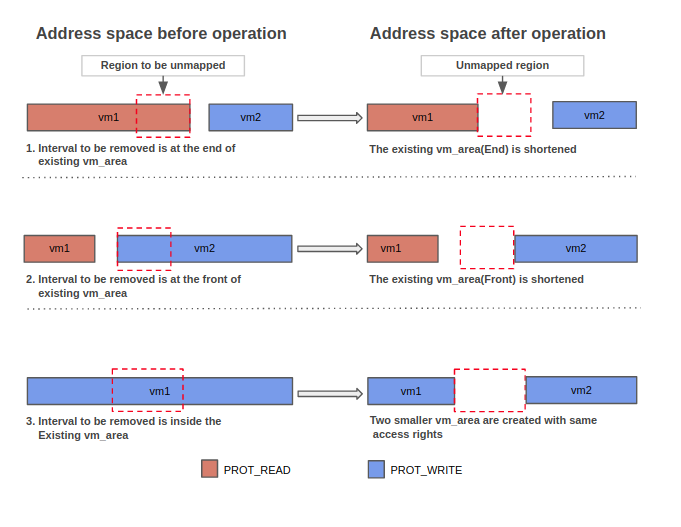
\includegraphics[width=14cm,height=12cm]{mm5.png}
    \caption{Unmapping of the VM area}
    \label{fig:my_label}
\end{figure}

\subsection*{\tt RETURN VALUE}
\noindent On success, {\tt munmap()} returns 0.  On failure, it returns -1 or {\tt EINVAL})

\newpage

\subsection *{\tt mprotect(void *addr, size\_t length, int prot)}
{\tt mprotect} changes the access protections for the calling process's memory pages containing any part of the address range in the interval  ({\tt addr}, {\tt addr}+ {\tt len}-1).  Assume that {\tt addr} provided as argument is always page aligned. {\tt mprotect} might create, expand or shrink the {\tt vm\_area} mapping(refer to the below figure).

\begin{figure}[H]
    \centering
    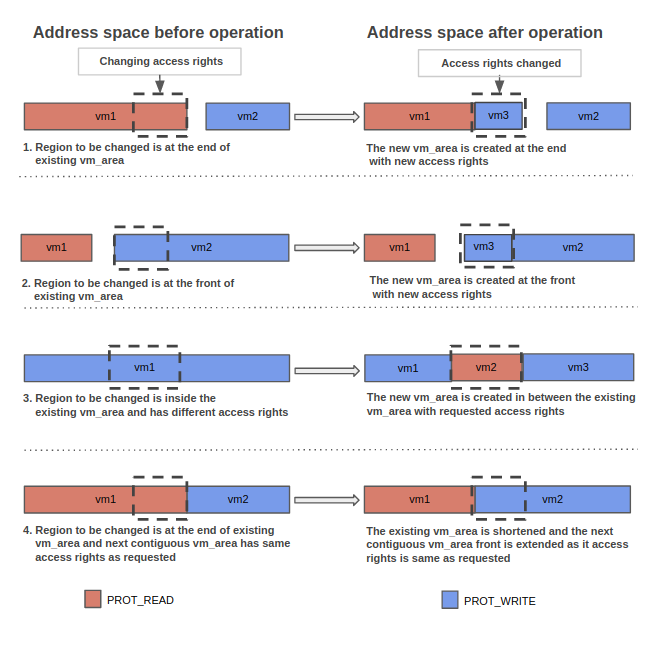
\includegraphics[scale=0.6]{mm6.png}
    \caption{Unmapping of the VM area}
    \label{fig:my_label}
\end{figure}

If the calling process tries to access memory in a manner that violates the protections, then the kernel generates a SIGSEGV signal for the process. As we are updating the access rights of certain regions in the {\tt vm\_area}, the access rights should also be updated accordingly in the underlying physical pages as well if they exist.
\newpage
The {\tt prot} argument describes the desired memory protection of the mapping.  It can be bitwise OR of one or more of the following flags:

    
    \begin{itemize}
        \item {{\tt PROT\_READ}  -  The protection of the mapping ({\tt vm\_area}) is set to {\tt READ\_ONLY}. The physical pages which map to this {\tt vm\_area} are also set to {\tt READ\_ONLY}. If any process tries to write on this physical page, it will result in {\tt SIGSEGV}}
        
        \item { {\tt PROT\_WRITE} - The protection of the mapping ({\tt vm\_area}) is set to {\tt WRITE\_ONLY}. When it comes to physical pages, {\tt PROT\_WRITE} implicitly provides read access to physical pages. Hence the physical pages which map to this {\tt vm\_area} will have {\tt READ\_WRITE} access.}
        
    \end{itemize}

\subsection*{\tt RETURN VALUE}
    On success, {\tt mprotect()} returns 0. If the provided {\tt addr} does belong to the existing {\tt vm\_area} mapping. then {\tt mprotect} will fail and returns either (-1) or ({\tt EINVAL})
\newpage
\subsection*{\tt cfork(void)}    
\texttt{cfork()} creates a new process by duplicating the calling process.  The new process is referred to as the child process.  The calling process is referred to as the parent process.

The  child and the parent process run in separate memory spaces.  At the time of \texttt{cfork()} both memory spaces have the same content. After \texttt{cfork()}, a write performed by parent or child results in copying of the page and thus child and parent stops sharing the page. 

The child and parent has separate user and kernel stack and memory areas shared by them till copy-on-write happens are data segment, mmaped regions. The child and parent continue sharing code region since it is read only regions.


The child process is an exact duplicate of the parent process except for the following points:
 \begin{itemize}
 \item The child has its own unique process ID.
 \item The child's parent process ID is the same as the parent's process ID.
 \end{itemize}
 
\subsubsection*{Example}
%\begin{small}
%\begin{lstlisting}
\begin{verbatim}
1. int main()
2.  {
3.      int pid;
4.      char * mm1 = mmap(NULL, 4096, PROT_READ|PROT_WRITE, 0);
5.      if(mm1 < 0)
6.      {
7.         printf("Map failed \n");
8.         return 1;
9.      }
10.      mm1[0] = 'A';
11.      pid = cfork();
12.      if(pid){
13.        mm1[0] = 'B';
14.        printf("mm1[0] inside parent:%c\n",mm1[0]);
15.      }
16.     else{
17.          printf("mm1[0] inside child:%c\n",mm1[0]);
18.     }
19.   }
\end{verbatim}

\begin{figure}[H]
    \centering
    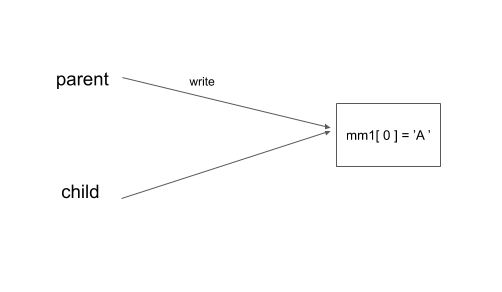
\includegraphics[scale=.5]{cfork.png}
    \caption{After parent called cfork()}
    \label{fig:cfork}
\end{figure}

After parent performs {\tt cfork}, the parent and child continues to share the memory regions as shown in figure \ref{fig:cfork}.

\begin{figure}[H]
    \centering
    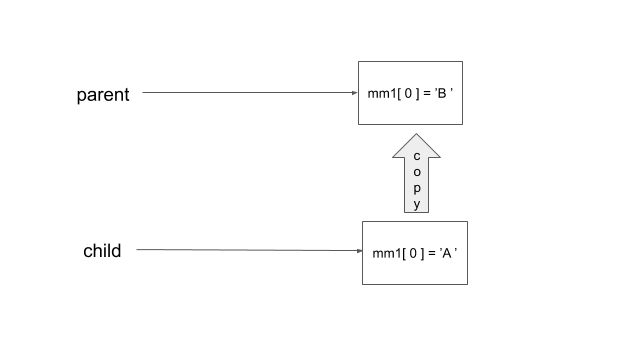
\includegraphics[scale=.5]{after_cfork.png}
    \caption{After parent writes}
    \label{fig:after_write}
\end{figure}

After {\tt cfork}, parent writes to the mapped area as shown in line number 13, which results in copy-on-write and child and parent stops sharing the memory area as shown in figure \ref{fig:after_write}. 

\begin{verbatim}
mm1[0] inside child:A
mm1[0] inside parent:B
\end{verbatim}

In the output shown above, as you can see, the child still sees the unmodified value where as the parent prints the new value.

\subsection*{\tt RETURN VALUE}

On success, the PID of the child process is returned in the parent, and 0 is returned in the child. On failure, -1 is returned in the parent, no child process is created, and errno  is  set appropriately.

\subsection*{\texttt{vfork(void)}}

\texttt{vfork()}, just like \texttt{cfork()}, creates a child process of the calling process. \texttt{vfork()} create new processes without copying the page tables of the parent process.

\texttt{vfork()} differs from \texttt{cfork()} in that the calling thread is suspended until the child terminates ( by calling exit(), or abnormally, after delivery of a fatal signal).  Until that point, the child shares all memory with its parent, including the stack.

The child and parent has separate kernel stack and memory areas shared by them till child exits are user stack, data segment, mmaped regions, and code.
 
\subsubsection*{Example}

\begin{verbatim}
1.int main()
2.{
3.   int pid;
4.   char * mm1 = mmap(NULL, 4096, PROT_READ|PROT_WRITE, 0);
5.   if(mm1 < 0)
6.   {
7.      printf("Map failed \n");
8.      return 1;
9.   }
10.   mm1[0] = 'A';
11.   pid = vfork();
12.   if(pid)
13.   {
14.      printf("mm1[0] inside parent:%c\n",mm1[0]);
15.   }
16.   else
17.   {
18.      mm1[0] = 'B';
19.      printf("mm1[0] inside child:%c\n",mm1[0]);
20.      exit(0);
21.    }
22.}
\end{verbatim}

\begin{figure}[H]
    \centering
    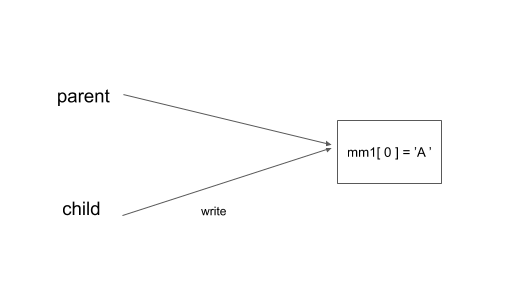
\includegraphics[scale=.5]{vfork.png}
    \caption{After parent called vfork()}
    \label{fig:vfork}
\end{figure}
After parent performs {\tt vfork}, the parent and child continues to share the memory regions as shown in figure \ref{fig:vfork}. The parent is in waiting state after {\tt vfork}, and child is ready for scheduling. The parent continues in waiting state until child exits.

\begin{figure}[H]
    \centering
    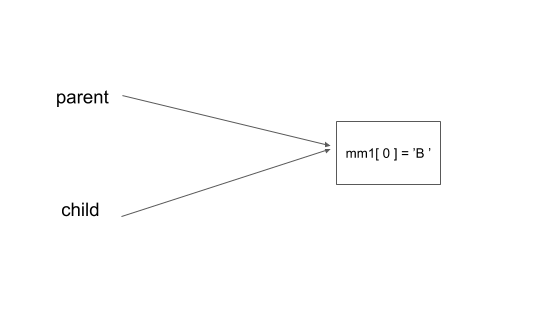
\includegraphics[scale=.5]{after_vfork.png}
    \caption{child writes and exits}
    \label{fig:vfork_after_write}
\end{figure}

After {\tt vfork}, child writes to the mapped area and exits by calling {\tt exit(0)}.
\begin{verbatim}
mm1[0] inside child:B
mm1[0] inside parent:B
\end{verbatim}
In the output shown above, as you can see, the parent prints the value which is written by the child.


\subsection*{\texttt{RETURN VALUE}}
On success, the PID of the child process is returned in the parent, and 0 is returned in the child. On failure, -1 is returned in the parent, no child process is created, and errno  is  set appropriately.

\newpage
\section*{Background and Utilities}
We have already provided a detailed specification of system calls that you need to implement. In order to make things easier, we have given some template functions, structures and a few utility functions that facilitate object creation and deletion. Lets have look at those functions.

The process control block (PCB) is implemented using a structure named {\tt exec\_context} defined in {\tt src/include/context.h}. One of the important members of {\tt exec\_context} for this assignment is the structure structure.

\subsection*{\tt struct vm\_area:}
\begin{itemize}
    \item[]
    \begin{itemize}
        \item[]
        \begin{itemize}
                \item[{\tt  vm\_start} -] The starting address (virtual address) of the {\tt vm\_area} mappings.
                \item[{\tt  vm\_end} -] The ending address (virtual address) of the {\tt vm\_area} mappings.
                \item[{\tt  access\_flags} -] The Protection or access flags of the current {\tt vm\_area} mappings.
                \item[{\tt  vm\_next} -] The pointer to the next {\tt vm\_area} mappings.
        \end{itemize}
    \end{itemize}
\end{itemize}


\subsection*{\tt struct vm\_area* alloc\_vm\_area():}
    This function is used to create a new {\tt vm\_area} mapping and returns a pointer to the created {\tt vm\_area}. We won't be filling or setting any values to members of the {\tt vm\_area}. You should only use this function to create {\tt vm\_area} in the entire assignment.

\subsection*{\tt void dealloc\_vm\_area(struct vm\_area *vm):}
    This function is used to delete or deallocate the {\tt vm\_area} which is passed as an argument. You should only use this function to delete or deallocate {\tt vm\_area} in the entire assignment.
    
\subsection*{ {\tt MMAP\_AREA\_START \& MMAP\_AREA\_END}:}
    These are constants defined in the file {\tt [src/include/mmap.h]} which is used to specify the overall start and end limit of the mmap space. All the mappings ({\tt vm\_area}) which are created using the mmap syscalls should reside within this limit. if the hint address is not within limit, then mmap syscalls should return {\tt EINVAL} or (-1).


\subsection*{\tt pmap(int details):}
    You can use the pmap methods to check the {\tt vm\_area} details. If {\tt details} is zero. Then pmap will print the count of {\tt vm\_area} and pagefaults for the address ranges between  {\tt MMAP\_AREA\_START} and {\tt  MMAP\_AREA\_END}. If {\tt details} is 1. Then pmap will dump the entire {\tt vm\_area} details.

\subsection*{\tt struct pfn\_info (in page.h)}

This object represents the physical memory page. The {\tt pfn\_info} for each page is maintained in {\tt list\_pfn\_info} object, which is indexed by the {\tt pfn} of physical memroy page.

{\tt pfn\_info} object has {\tt refcount} which is used to maintain count of number of sharers for a physical memory page. This count helps to identify whether to copy a page at the event of a write after {\tt cfork()}. The page needs to be copied when number of sharers is greater than one.

\subsection*{\tt get\_pfn\_info(u32 index) (in page.c)}
 You can make use of this function to get {\tt pfn\_info} object corresponding to a {\tt pfn} of physical memory page.
 
\subsection*{\tt increment\_pfn\_info\_refcount(struct pfn\_info * p)(in page.c)}
 You can use this method to increment refcount of a physical memroy page at the time of {\tt cfork()}.
\subsection*{\tt decrement\_pfn\_info\_refcount(struct pfn\_info * p)(in page.c)}
 You can use this method to decrement refcount of a physical memroy page at the time of copy-on-write after a {\tt cfork()}.
 
\subsection*{\tt get\_pfn\_info\_refcount(struct pfn\_info *p)(in page.c)}
This method gives current refcount of a physical memroy page.

\subsection*{\tt format of Page Table Entry}
The format of PTE entry which maps to 4KB pages in intel x86 architecture is as shown in figure \ref{fig:pte}. Those who want to know more, can refer \href{https://software.intel.com/sites/default/files/managed/39/c5/325462-sdm-vol-1-2abcd-3abcd.pdf}{Intel Software Manual} (page 2831).
\begin{figure}[H]
    \centering
    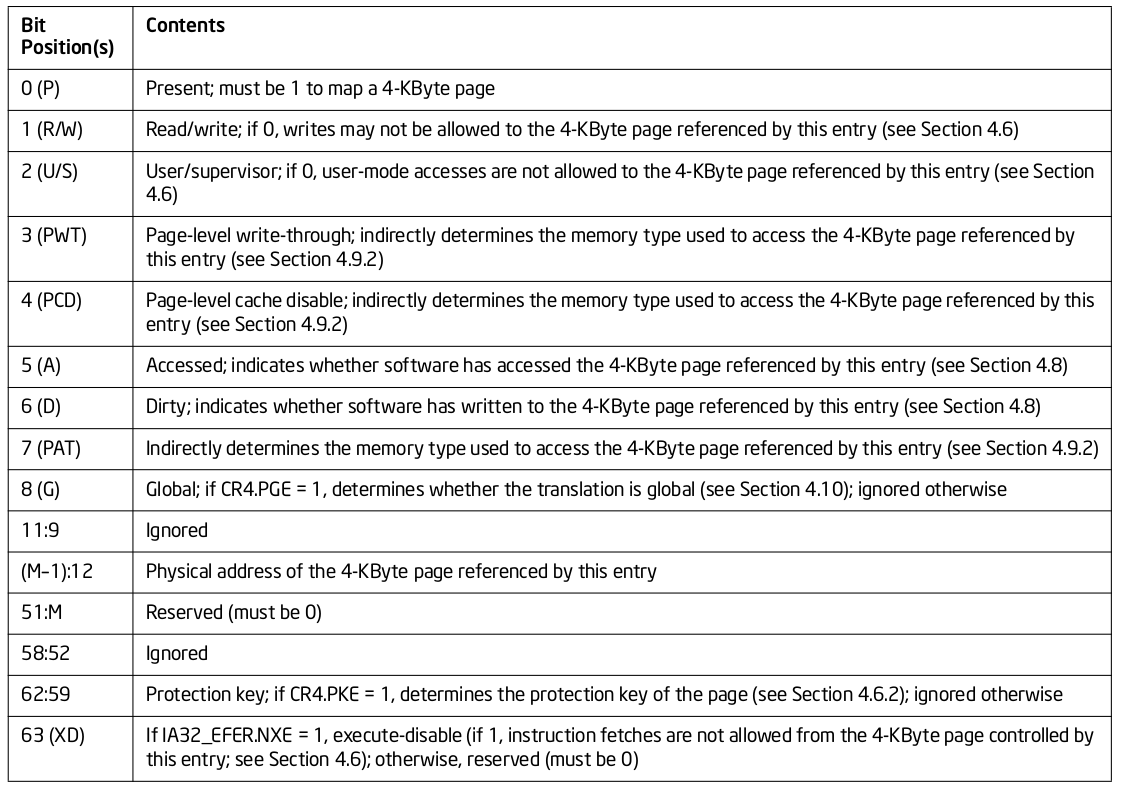
\includegraphics[scale=.25]{PTE_Entry.png}
    \caption{PTE Entry}
    \label{fig:pte}
\end{figure}

For this assignment, you can ignore bit positions 3-11 and 51-63. You only need to modify bit positions 0, 1, 2 and 12-50.

\subsection*{\tt Page-Fault Error Code}
The error codes in intel x86 architecture incase of a page fault is as shown in figure\ref{fig:pagefault}, which is taken from course slides. User-mode read access to an unmapped page results in error code 0x4, same way user-mode write access to an unmapped page results in error code 0x6. The error code 0x7 indicates user mode write access to read-only page which has page table mapping. Those who want to know more, can refer \href{https://software.intel.com/sites/default/files/managed/39/c5/325462-sdm-vol-1-2abcd-3abcd.pdf}{Intel Software Manual} (page 2836).
For this assignment, you need to only modify P, W, U bits.
\begin{figure}[H]
    \centering
    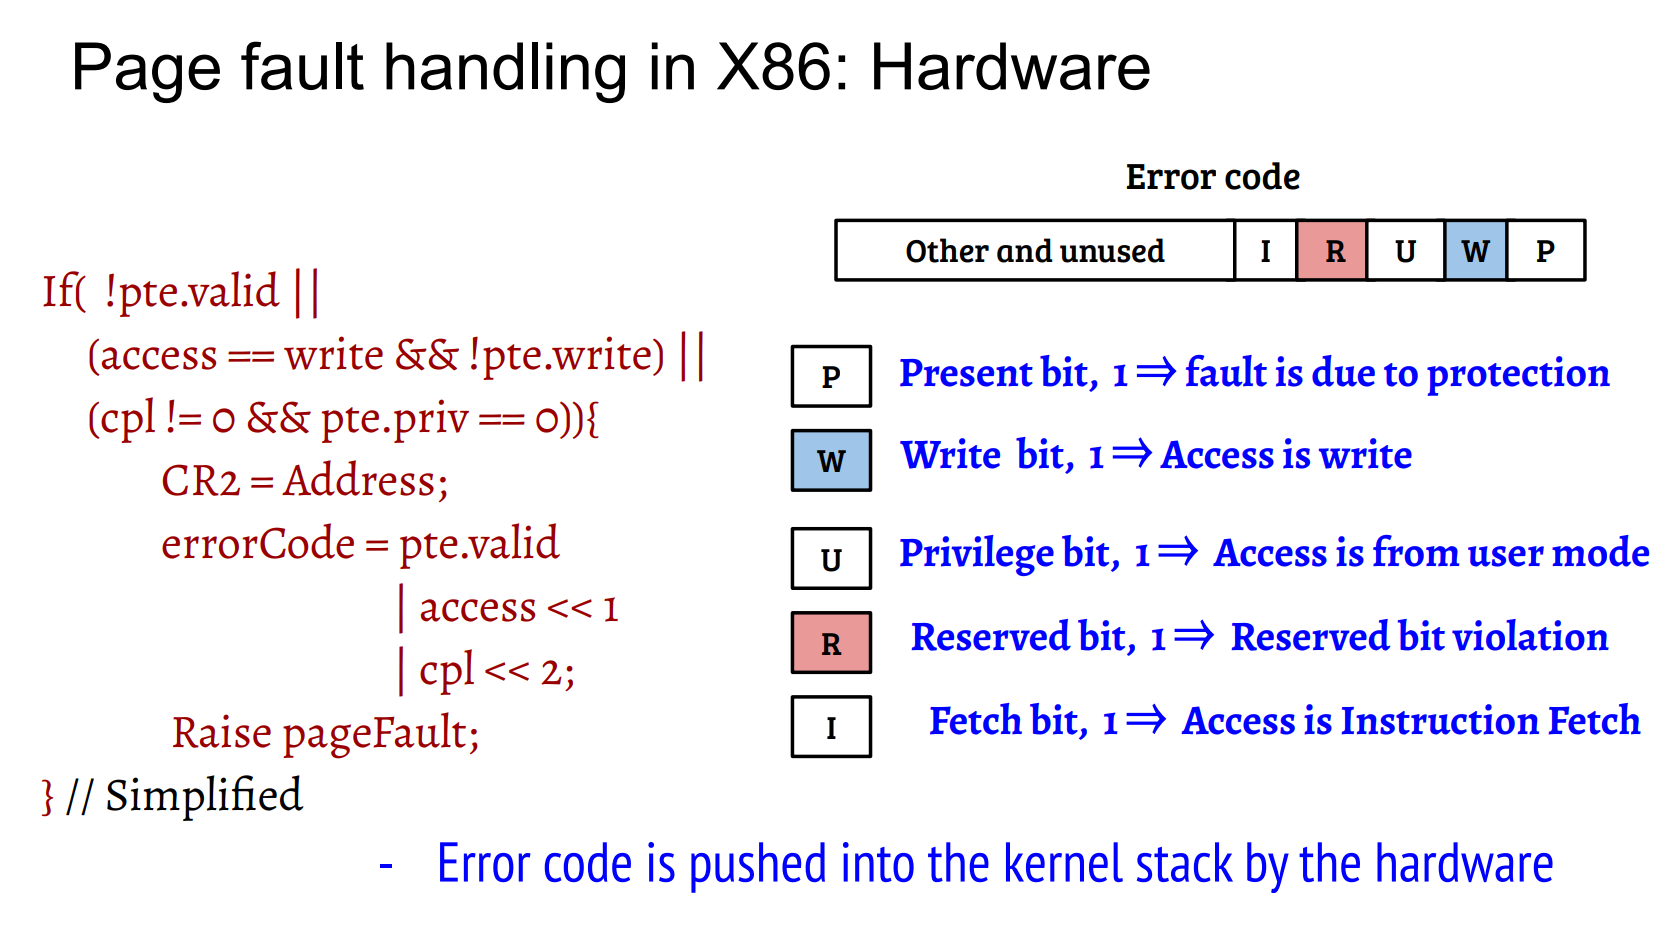
\includegraphics[scale=.25]{Errors.png}
    \caption{Page-Fault Error Code}
    \label{fig:pagefault}
\end{figure}


\newpage
\section*{Task-1: Virtual memory area operations (30 Marks)}


\subsection*{\tt mmap():}
    To implement {\tt mmap} system call, you are required to provide implementation for the template function {\tt vm\_area\_map} in the file {\tt [src/mmap.c]}) which takes the current context, address, length, protection and flags as arguments. You are supposed to maintain all the {\tt vm\_area} mappings in the singly linked list data structures. The head of singly linked list is inside the current context({\tt current->vm\_area}).
    
    Based on the request and the hint address, You might be creating (adding a node in singly linked list), shrinking, expanding and merging the {\tt vm\_area} in the singly linked list (refer the specification mmap). To create and delete use {\tt alloc\_vm\_area} and {\tt dealloc\_vm\_area} respectively.
    
\subsection*{\tt munmap():}
     To implement {\tt munmap} system call, you are required to provide implementation for the template function {\tt vm\_area\_unmap} in the file {\tt [src/mmap.c]}) which takes the current context, address, length as arguments. Based on the address and length, You might be deleting and shrinking the ({\tt vm\_area}) mappings in the singly linked list (refer the munmap specification).
     
\subsection*{\tt mprotect():}

      To implement {\tt mprotect} system call, you are required to provide implementation for the template function {\tt vm\_area\_mprotect} in the file {\tt [src/mmap.c]}) which takes the current context, address, length and protection as arguments. 
      
      If the provided address is not part of any {\tt vm\_area}. Then mprotect will fail the request and return {\tt EINVAL} or (-1). Based on the request, You might be creating ,shrinking, expanding and merging the {\tt vm\_area} in the singly linked list (refer the specification mprotect).

\subsection*{\tt Validation Procedure:}

    \begin{itemize}
        \item In this part of the assignment we won't be validating anything regarding physical pages( mapping physical page, updating page table, page fault handling)
        \item We will only be validating the state of {\tt vm\_area}(nodes in the single linked list) such as number of {\tt vm\_area} before and after the syscall operations.
        \item There can be at most 128 {\tt vm\_area} at any point of time. If not then return EINVAL or -1.
        \item The address ranges for all the above system call should be between the address ranges {\tt MMAP\_AREA\_START \& MMAP\_AREA\_END}. If not then return EINVAL or -1.
        \item We will be checking the {\tt vm\_area} protection or access rights.
        \item Assume all the address provided to the syscalls are page-aligned.
         
    \end{itemize}


\newpage
\section*{Task-2: Assigning physical pages (30 Marks)}

We have provided a template function {\tt vm\_area\_pagefault} which takes the current context, address (faulted address) and error code. This function will be called whenever there is read page fault ({\tt error\_code} will 4) and write page fault ({\tt error\_code will be 6}) in mmap addresses ranging between {\tt MMAP\_AREA\_START} and {\tt MMAP\_AREA\_END}. 

For valid access, map a physical page and function should return 1. For invalid access (Write fault on the address which maps to read only {\tt vm\_area}) function should return -1.

\subsection*{\tt mmap()}
    If a {\tt vm\_area} mapping is created without providing a  {\tt MAP\_POPULATE} flags. Then all the subsequent access to the {\tt vm\_area} mapping will result in page fault (Lazy allocation).The {\tt vm\_area\_pagefault} function will be called in case of page fault. You have to map physical page, set access flags and update page table entries of the faulted address.
    
    If  a {\tt vm\_area} mapping is created with {\tt MAP\_POPULATE} flags. Then you have to map physical page, set access flags and update page table entries at the time of {\tt vm\_area} creation,  Any access to the {\tt vm\_area} mapping is created with {\tt MAP\_POPULATE} flags should not result in page fault.

\subsection*{\tt munmap()}
    On unmapping a {\tt vm\_area} mapping, if a {\tt vm\_area} has physical pages mapped to it then you have to unmap the physcial pages and update the page tables accordingly.

\subsection*{\tt mprotect()}
    On changing the protection or access rights of  {\tt vm\_area} mappings, if a {\tt vm\_area} has physical pages mapped to it. Then you have to update the access rights as the physical page as well.


\subsection*{\tt Validation Procedure:}
     \begin{itemize}
        \item We will be validating state of {\tt vm\_area}, number of page faults, access right of physical pages and {\tt vm\_area}.
        \end{itemize}
        
\newpage

\section*{Task-3: Smart Process Creation (40 Marks)}

\subsection*{\tt cfork()}
{\tt cfork}(copy on write fork) creates a new process by duplicating the calling process. The new process is called {\tt child } process and the calling process is called {\tt parent}. The {\tt child} process and {\tt parent} process run in separate memory spaces. The {\tt child} and {\tt parent} share physical memory pages till either of them modifies it. The page is mapped as read-only to both parent and child initially and at the event of a write, copy of the page is created and PTE entry is updated to point to new page.

 
As part of this task, you need to implement {\tt cfork\_copy\_mm}(in cfork.c). The functionality of {\tt cfork\_copy\_mm} is to setup page table for the child. The page table entries for the {\tt child} point to the same physical pages of the {\tt parent} on copy-on-write basis. You need to mark pages are readonly (so that write to these pages can be identified to trigger copy-on-write) by clearing R/W bit in PTE entry of child and parent page table (0 value at R/W bit indicates writes may not be allowed to the 4-KByte page referenced by this entry). You can use {\tt install\_ptable}(in context.c) to setup page table for the {\tt child}. The {\tt child} will share all memory segments and vm areas of {\tt parent} on copy-on-write basis except for user stack area, {\tt child} has a separate user stack from that of {\tt parent}.

You also need to implement {\tt handle\_cow\_fault}(in cfork.c) which will be called from {\tt do\_page\_fault} incase of a copy-on-write fault ({\tt error\_code will be 7}). In {\tt handle\_cow\_fault}, you should ensure that the faulting address({\tt cr2}) is in a valid range and write is allowed as per {\tt access\_flags} of faulting segment/vm area. 

{\tt cfork\_copy\_mm} will be called from {\tt do\_cfork}(in entry.c). The {\tt do\_cfork}(in entry.c) gets a new {\tt exec\_context}
and copies {\tt current} execution context. The {\tt do\_cfork} finally calls {\tt setup\_child\_context} to create os stack and make {\tt child} ready for scheduling.

Please note that there is no ASID support in the system, so the TLB entries should be handled accordingly.

\subsection*{\tt Validation Procedure:}		
     \begin{itemize}		
        \item We will check number of copy-on-write page faults.		
        \item We will check number of pages before and after a write followed by {\tt cfork()}.		
        \end{itemize}

\subsection*{\tt vfork()}

{\tt vfork} is same as {\tt cfork}. {\tt vfork} differs from {\tt cfork} in that the calling process is suspended until the child terminates by calling {\tt exit()}. Until that point, the child shares all memory with its parent, including the stack. The child must not return from the current function and should call {\tt exit()} in user code. The child process should take care not to modify the memory in unintended ways, since such changes will be seen by the parent process once the child terminates.

			
As part of this task, you need to implement {\tt vfork\_copy\_mm} (in cfork.c) which is called from {\tt do\_vfork} (in entry.c). The functionality of {\tt vfork\_copy\_mm} is to make the child use parent's page table.

The {\tt child} will share all memory segments and vm areas of {\tt parent} including the user stack. You need to make sure that, the child does not overwrite user stack entries of parent to ensure correct execution of parent after child exits. You can overwrite the {\tt entry\_rsp} and {\tt rbp} in {\tt user\_regs} which is present in {\tt exec\_context}(in context.h) of the process to manipulate user stack position, since these values are loaded to hardware registers by {\tt schedule}(in schedule.c) at the time of process schedule.

The {\tt parent} state should be changed to WAITING before scheduling {\tt child} by calling {\tt schedule(new\_ctx)} in {\tt do\_vfork}.

When the {\tt child} exits, change state of {\tt parent} to READY in {\tt vfork\_exit\_handle} (in cfork.c), which is called from {\tt do\_exit} (in entry.c).
\subsection*{\tt Validation Procedure:}
     \begin{itemize}
     \item We will check sharing of page table between parent and child.
     \item We will check that parent is waiting till child exits.
     \end{itemize}

\section*{Submission guidelines}
\begin{itemize}
\item The assignment is to be done individually. You have to submit only two files (mmap.c and cfork.c). Put these two files in a directory named with your roll number. Create a zip archive of the directory and upload in canvas.
\item {\em Don't modify any other files}. We will not consider any file other than {\tt mmap.c} and {\tt cfork.c} for evaluation.
\item {\em You should remove all printf/prink debug statements from submission files}. We will taking diff of your output and expected output
for evaluation.
\end{itemize}


In-case of any issues you should reach out to us at the earliest.  All the best!

\end{document}
